\documentclass[reqno,openany,12pt]{amsbook}
\usepackage{amsmath}
\usepackage[pdftex]{graphicx}

\usepackage{tikz}
\usetikzlibrary{mindmap,trees}
%  openany option dumps the blank pages between chapters when the next
%  chapter starts on odd page number; following command had similar
%  effect
%  \let\cleardoublepage\clearpage
%  NB need an abstract or get a blank page between title and contents


\renewcommand{\baselinestretch}{1.35}


%  ************  begin my definitions  *******************

% *** theorem etc. commands ***

\newtheorem{thm}{Theorem}%[section]
\newtheorem{lemma}[thm]{Lemma}
\newtheorem{cor}[thm]{Corollary}

\theoremstyle{definition}
\newtheorem{definition}[thm]{Definition}
\newtheorem*{ass}{Assumption S}

\theoremstyle{remark}
\newtheorem{remark}[thm]{Remark}

%\numberwithin{equation}{section}

\newenvironment{mylist}{\begin{enumerate}
\def\labelenumi{\theenumi}
\renewcommand{\theenumi}{(\roman{enumi})}
}{\end{enumerate}}

% *** greek commands ***

\newcommand\al{\alpha}
\newcommand\be{\beta}
\newcommand\ga{\gamma}
\newcommand\Ga{\Gamma}
\newcommand\de{\delta}
\newcommand\De{\Delta}
\newcommand\ep{\epsilon}
\newcommand\ka{\kappa}
\newcommand\la{\lambda}
\newcommand\La{\Lambda}
\newcommand\om{\omega}
\newcommand\Om{\Omega}
\newcommand\si{\sigma}
\newcommand\Si{\Sigma}
\renewcommand\th{\theta}
\newcommand\Th{\Theta}

% *** tilde/bar/bold commands ***


\newcommand\bg{\bar g}
\newcommand\bh{\bar h}
\newcommand\bu{\bar u}

\newcommand\bq{\boldsymbol{q}}
\newcommand\br{\boldsymbol{r}}
\newcommand\bv{\boldsymbol{v}}

% *** Bbb commands ***

\newcommand\Q{\mathbb{Q}}
\newcommand\R{\mathbb{R}}
\newcommand\Nf{\mathbb{N}}
\newcommand\Zf{\mathbb{Z}}

% *** script commands ***

\newcommand\I{{\mathcal I}}

\newcommand\B{{\mathcal B}}

% *** brackets commands ***

\newcommand\lan{\langle}
\newcommand\ran{\rangle}

% *** various maths commands ***

\newcommand\X{\times}
\newcommand{\tow}{\rightharpoonup}
\newcommand{\pa}{\partial}
\newcommand\rot{{\rm Rot}}


%  ************  end my definitions  *******************


\begin{document}


\title{Masters in Computer Vision\\Software Engineering Project\\2013-2014}
\author{Ozan\\Oksana\\Klemen\\Natalia\\
{\small
January 2014
}
}
\bigskip



%\begin{abstract}
%This project will investigate some aspects of rational approximation to
%real numbers.
%It is well known that any irrational number can be estimated arbitrarily
%close by rationals, i.e. for any $\ep>0$ and irrational $x \in \R$,
%there exists integers $p$,$q$ such that
%\begin{equation}  \label{abs_basic_app.eq}
%\left| {x-\frac{p}{q}} \right| < \ep
%\end{equation}
%This is known as Diophantine approximation, named after Diophantus of
%Alexandria.
%
%\end{abstract}


\maketitle


 \setcounter{page}{0}


\tableofcontents


\chapter{Introduction}

As a project at Software Engineering class we had to develop an application that to some extent mimics well known Google Earth. The main idea is to give an user who is unfamiliar with Le Creusot the tool that enables him to search for shortest path between two points on the map, enables him to create an itinerary containing different types of points of interest. We had to do all this in C++ and in Matlab.

\chapter{Project management}
In this chapter we want to present how our group organized and managed this project. As we all had a bit of software designing experiences, we knew how important a proper plan and research before the implementation is. Unfortunately, we were also aware that no matter how good the plan is, we will be forced to adjust it during the implementation, because of the things we did not take into account while planning or because some things turned out to be different to what we assumed. Because of that we decided to follow the iterative and incremental development model, which enabled us to adjust our plans after each of the implementation iterations. A schematic representation of the iterative and incremental development model can be seen on figure \ref{fig:Iterative_development_model_V2}. 
\begin{figure}[h]
\centering
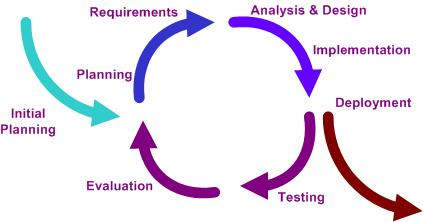
\includegraphics[height=4cm]{../photos/Iterative_development_model_V2}
\caption{An iterative development model}
\label{fig:Iterative_development_model_V2}
\end{figure}
\section{Basic building blocks}
To be able to fully manage the project at all times we decided to split the project into four main parts:
\begin{itemize}
\item User interface
\item Database
\item Map representation
\item Path algorithms
\end{itemize}
\begin{tikzpicture}
  \path[mindmap,concept color=gray,text=white]
    node[concept] {Project}
    [clockwise from=0]
    child[concept color=green!60!black] {
      node[concept] {User interface}
    }  
    child[concept color=blue] {
      node[concept] {Map representation}
    }
    child[concept color=red] { node[concept] {Path algorithms} }
    child[concept color=orange] { node[concept] {Database} };
\end{tikzpicture}
\subsection{UI - User Interface}\hspace*{\fill} \\
It is the part of the application that is responsible for user interaction with the application. Main goal is to make the interface as user-friendly as possible. In the beginning we made a rough sketch of how the interface should look (figure []), but we, as expected, changed it a little bit during the development. The UI is presented more in details in chapter [UI USER MAUNAL].
\subsection{Database}\hspace*{\fill} \\
Our database consists of two parts. The static part, having the information about the roads in Le Creusot (described in []) and the dynamic part with the information about the points of interest. From the beginning we were deciding between using XML based and relational database. During the consideration we took into account the following facts:
\begin{itemize}
\item Most of the data is static - information about the roads in Le Creusot will not change;
\item Dynamic data will change rarely - user will not often update information about the points of interest;
\item Relatively small amount of data - Le Creusot is a small city, so there is not a lot of information about the roads. This gives us the opportunity to read all the information to memory at the beginning, reducing the latency caused by queries to the database;
\item Easiness of install and mobility -  using relational database, requires installation of different software (sql server, connectors, etc.) on the clients computer, which we wanted to avoid. 
\end{itemize}  
Because of all these reasons we decided to use XML based database. We have the information about the roads in one osm file, while the information about the points of interest is in xml file. We will describe both of them more  in detail in later chapters.
\subsection{Map representation}\hspace*{\fill} \\
TODO
\subsection{Path algorithms}\hspace*{\fill} \\
This part consists of all calculations about paths, distances, travelling times and optimizations of the paths. Our main goal is to make the algorithms work as quickly as possible, taking into account all the restrictions road networks has (oneway streets, footways etc.). We also want to make the algorithms as reusable as possible, to reduce the redundancy in development and minimize the possibilities of errors.
\section{Meetings and Project Progress}

Development stages can be divided in three parts. First stage included analysing the problem, extracting project requirements and devising a plan for the implementation. Second part included extracting the application structure, collecting most appropriate tools for the implementation and setting up the environment. The last part is the implementation itself starting from building the basic blocks, simple prototype application and then gradually adding functionalities and features, alongwise with documenting the software. All the stages were supported with meetings according to time constraints and project progress speed.

\subsection{Analysing the problem}
Fist meetings were devoted to the analysing the provided requirements and inventing all possible useful features. Besides the general idea of user interface was developed according to all the needed functionality of the project. The scope of the project was defined and future work planned.

\subsection{Pre-implementation stage}
In the later meetings we were considering architecture challenges and possible solutions, able to provide the need functionality for the application. We were focusing on extracting the most appropriate tools and libraries to ease the development process as well as getting the idea . After it was done the same development environment was set up on all the computers. At this point it was clear how the implementation will differ in Matlab and C++ and the team got slitted between Matlab and C++ development.

\subsection{Implementation}
All next meetings were devoted to the coding the application and solving particular issues. At this stage separate basic blocks (ui, map-rendering, database, algorithms) were developed and then merged in one working application prototype, which only consisted of two-point path search. When it was clear that all the framework decisions were reasonable, further development was done.

\subsection{Software used for project management}
At first and second stage Dropbox was used to share latest meeting reports, schematics, useful papers and links. On the last stage the need of tool for simultaneous development became obvious. For that purpose, we chose GitHub repository hosting service. Besides, it was extremely useful for tracking issues and bugs. At very last meetings we used Skype conferences, since all the project team members were in different places.

\chapter{Initial planning}
As already mentioned in the previous chapter, we decided to use the iterative and incremental development model. Before starting the iterations we spend quite a lot of time on the initial planning, with special attention to user and general project requirements analysis. From the project's instructions we were able to identify the following major user requirements and construct use case diagram:
\begin{itemize}
\item user should be able to enter start and end point either by:
\begin{itemize}
\item mouse click
\item specifying latitude and longitude
\item selecting a point of interest
\end{itemize}
\item find shortest path from point A to point B (by foot or by car)
\item find all points of interest in a certain radius from point A (by foot or by car)
\item construct an itinerary from point A to point B with points of interest in between (with max distance limit)
\item view, edit and add points of interest (POI)
\end{itemize}
For better 
\section{Shortest path A -> B}
\section{title}
!!!ADD image of the use case diagram
\chapter{Plan of implementation}
After having the user requirements, we decided to make the global plan of implementation. Here we had to take into account, that we have to develop the application in C++ and Matlab. As show in the figure[] we have already splited  the project into four main parts. Because the user interface and map representations require completely different approaches in C++ and Matlab, we decided to split them into two parallel projects, one almost independent from another. On the other hand, we decided to use the same algorithms for both projects. The main reason was to minimize the redundancies in the research and development stage and minimize the possibility of errors. This way we could have the same algorithms for both, differing only in pure implementation details. \\
\\ Each of was delegated to oversee one of the parts (as shown in figure []). We have to emphasis that this does not mean he/she developed that part by him/herself, not even that he is solely responsible for it. No matter the delegation, we all worked on all parts of the project, either in research, design or implementation stage.
TODO: ADD IMAGE OF PARTS WITH DELEGATION
\section{MAYBE TIME PLAN?}
\chapter{Data}
Our application uses two main types of information. \textit{Static} map data describing the streets and \textit{dynamic} data about the different points of interest (POIs). The difference between static and dynamic data lies in the users ability to add and edit POIs data, while the map information is not meant to be changed by the user. \\
\\ The acquisition of this data was not the essence of the project, so we were allowed to use any data source, with appropriate licence and collaborate with other groups. 
\section{Map data}
Acquisition of map data (street locations, street types, buildings etc.) can be extremely time consuming and can easily produce not reliable results. At the same time, there is a lot of different open source data available on-line. Together with the other groups we decided to use OpenStreetMap data by the OpenStreetMap Foundation[].\\
\\
OpenStreetMap is an open source project providing free map data of the world. Data is published under the \textit{Open Database License (ODbL) from Open Data Commons (ODC)}, which enables us to freely produce the works from the database, modify, transform and build upon the database.
\subsection{Data format}
OpenStreetMap data consists of four core elements:
\begin{itemize}
\item Nodes - are basic point of location. They consist of longitude and latitude information. They can be used as a single point (POI) or ia a list of nodes (way);
\item Ways - ordered list of nodes, representing a street, an area (lake, forest etc.);
\item Relations - ordered list of nodes and ways which can be in a relation (many roads can be included in a long motorway);
\item Tags - key-value pairs which are used to store information about different objects (nodes, ways, relations)
\end{itemize}
Figure \ref{fig:Osm_flow} shows the difference between them.
\begin{figure}[h]
\centering
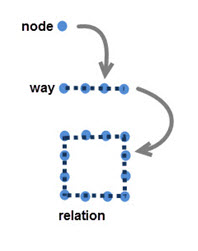
\includegraphics[height=4cm]{../photos/OSM_flow.jpg}
\caption{An iterative development model}
\label{fig:Osm_flow}
\end{figure}

\section{Points of Interest (POI)}
One of the main requirements for our application is to enable user to search using different points of interest. For aquisition of this points, all of the groups again collaborated, each marking all the points in part of Le Creusot. For each point we decided to acquire:
\begin{itemize}
\item name;
\item location;
\item address;
\item photo.
\end{itemize}
In the end we also categorized all the points into 26 different categories. 

\section{Database}
As described, our data consists of two parts. Static map data and dynamic points of interests data. For the beginning, we were deciding between using relational database and XML based database. With each of them having some benefits, we took during the consideration into account the following facts:
\begin{itemize}
\item Most of the data is static - information about the roads in Le Creusot will not change;
\item Dynamic data will change rarely - user will not often update information about the points of interest;
\item Relatively small amount of data - Le Creusot is a small city, so there is not a lot of information about the roads. This gives us the opportunity to read all the information to memory at the beginning, reducing the latency caused by queries to the database;
\item Easiness of install and mobility -  using relational database, requires installation of different software (sql server, connectors, etc.) on the clients computer, which we wanted to avoid. 
\end{itemize} 
In the end we decided to use \textbf{XML based database}. We kept the two parts od the data splitted into separate xml files. We kept the OpenStreetMap data in the osm files and created another XML file for POI data. This way, we could easily change th () This separation enables us to easily change either the either map data or the POI data.
\\ IMAGE OF DB FILES
\\Using XML based database produced one big disadvantage, which we had to take into account. XML based database is saved in a single file, which does not provide the ability to easily update POI data. Unfortunately, every time we update this data, we have to rewrite the whole file. This can in some occasions be the source of problems, as the writing to the file can be disrupted or cancelled, making the file unusable. However, we do not anticipate the user to update the data frequently, so we took this compromise.
 
 \chapter{Data structure}
 We have designed out class structure with the A* algorithm for the shortest path and OpenStreetMap (OSM) file structure in mind. We followed the OSM structure, having a basic class called \textbf{Node}. In figure \ref{fig:types_db} we show the different types we use with a small graphic representation.
 \begin{figure}[h]
 \centering
 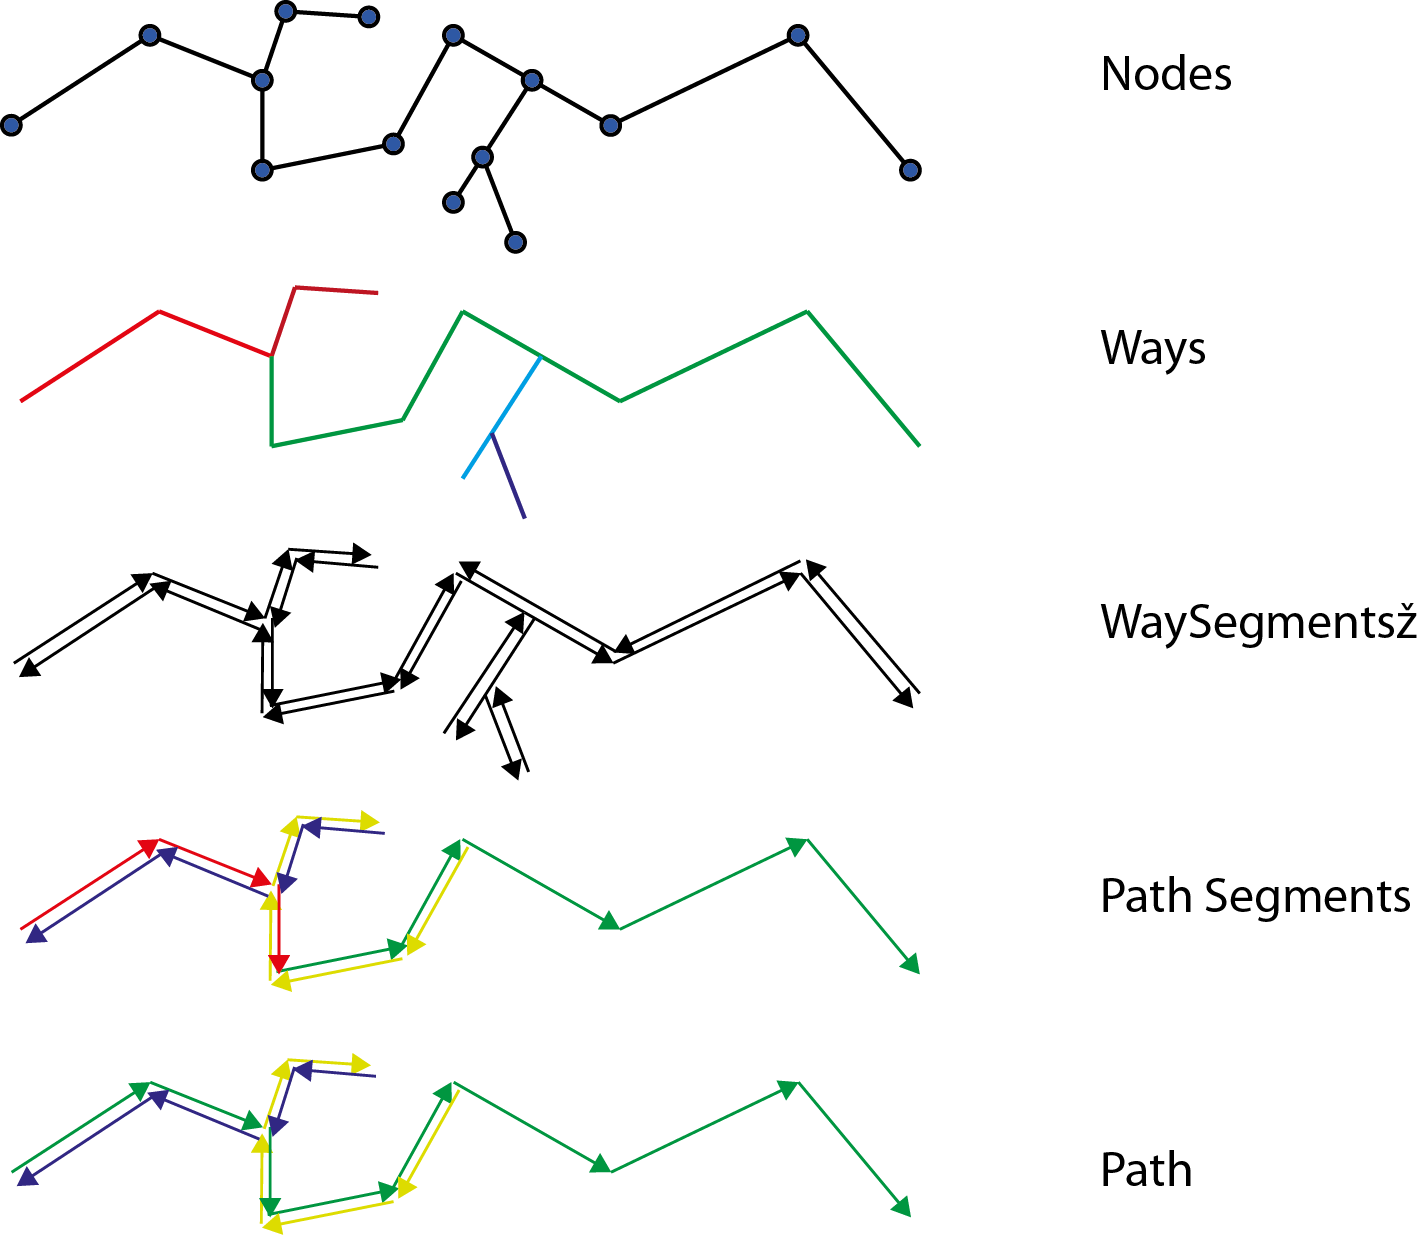
\includegraphics[height=4cm]{../photos/ways.png}
 \caption{Different objects in our data structure}
 \label{fig:types_db}
 \end{figure}
  \textbf{Node}
\\It is used to represent a single point on the map. This can either mark a point of interest (POI), or can be a part of a Relation such as \textit{way segment, building or way}. It contains location information, some A* algorithm informations (weights, visited, etc.) and a vector of Way Segments to which we can access from this Node. This is important expecially for A* algorithm, as it significantly reduce the time needed to find all possible and subsequently the correct next move.
\\
\textbf{Way}\\
Class implemented as in OSM file, to store the properties of each of the ways. It us usually used to represent whole streets, or part of the streets that have the same properties. Each way is assigned a type (primary, secondary, etc.), direction (oneway, bidirectional) and access privilages (private or public).\\
\textbf{Relation}
Relation is a base class from which we extend different relations (WaySegment, Building). It only contains a vector of pointers to Nodes that are in one specific relation and type of the relation.\\
\textbf{WaySegment}
Way Segment is the base class for our path algorithms. Way segment connects two nodes in a specific direction. This means that if the road between two nodes is bidirectional, we will create two WaySegments, one for each direction. We also have a pointer to an object Way which the road traversing belongs to. This gives us the option of getting information about the road at any time.
\\
\textbf{Path Segment}\\
It is a class that is used to store the result of a \textit{shortest path search}. It contains all the pointers to WaySegment objects we need to traverse in order to get from point A to point B. \\
\textbf{Path}\\
Object that contains vector of PathSegment pointers. Path is the end result of any search. If the search is solely path from point A to B, the path is going to have one PathSegment pointer. On the other hand, if we search for intinerary, Path will indluce multiple PathSegments, one for each pair of middle points.
\\
\textbf{Database}\\
Database is an base class for the whole database. It contains functions for correct parsing of XML files and also contains containers \textit{(std::map)} with pointers to each of the class created. We use this to quickly retrieve the classes based on their ID, and to be sure to delete all created objects in the destructor of the class. We also used a boost implementation of a \textit{rtree} data structure to hold all the WaySegment objects to quickly find all the WaySegments in a neighborhood of a point. This is very useful in implementation of finding the closest waySegment.
\\
In figure \ref{fig:db_class} we can see the whole class diagram of the database part of the application in C++.
 \begin{figure}[h]
 \centering
 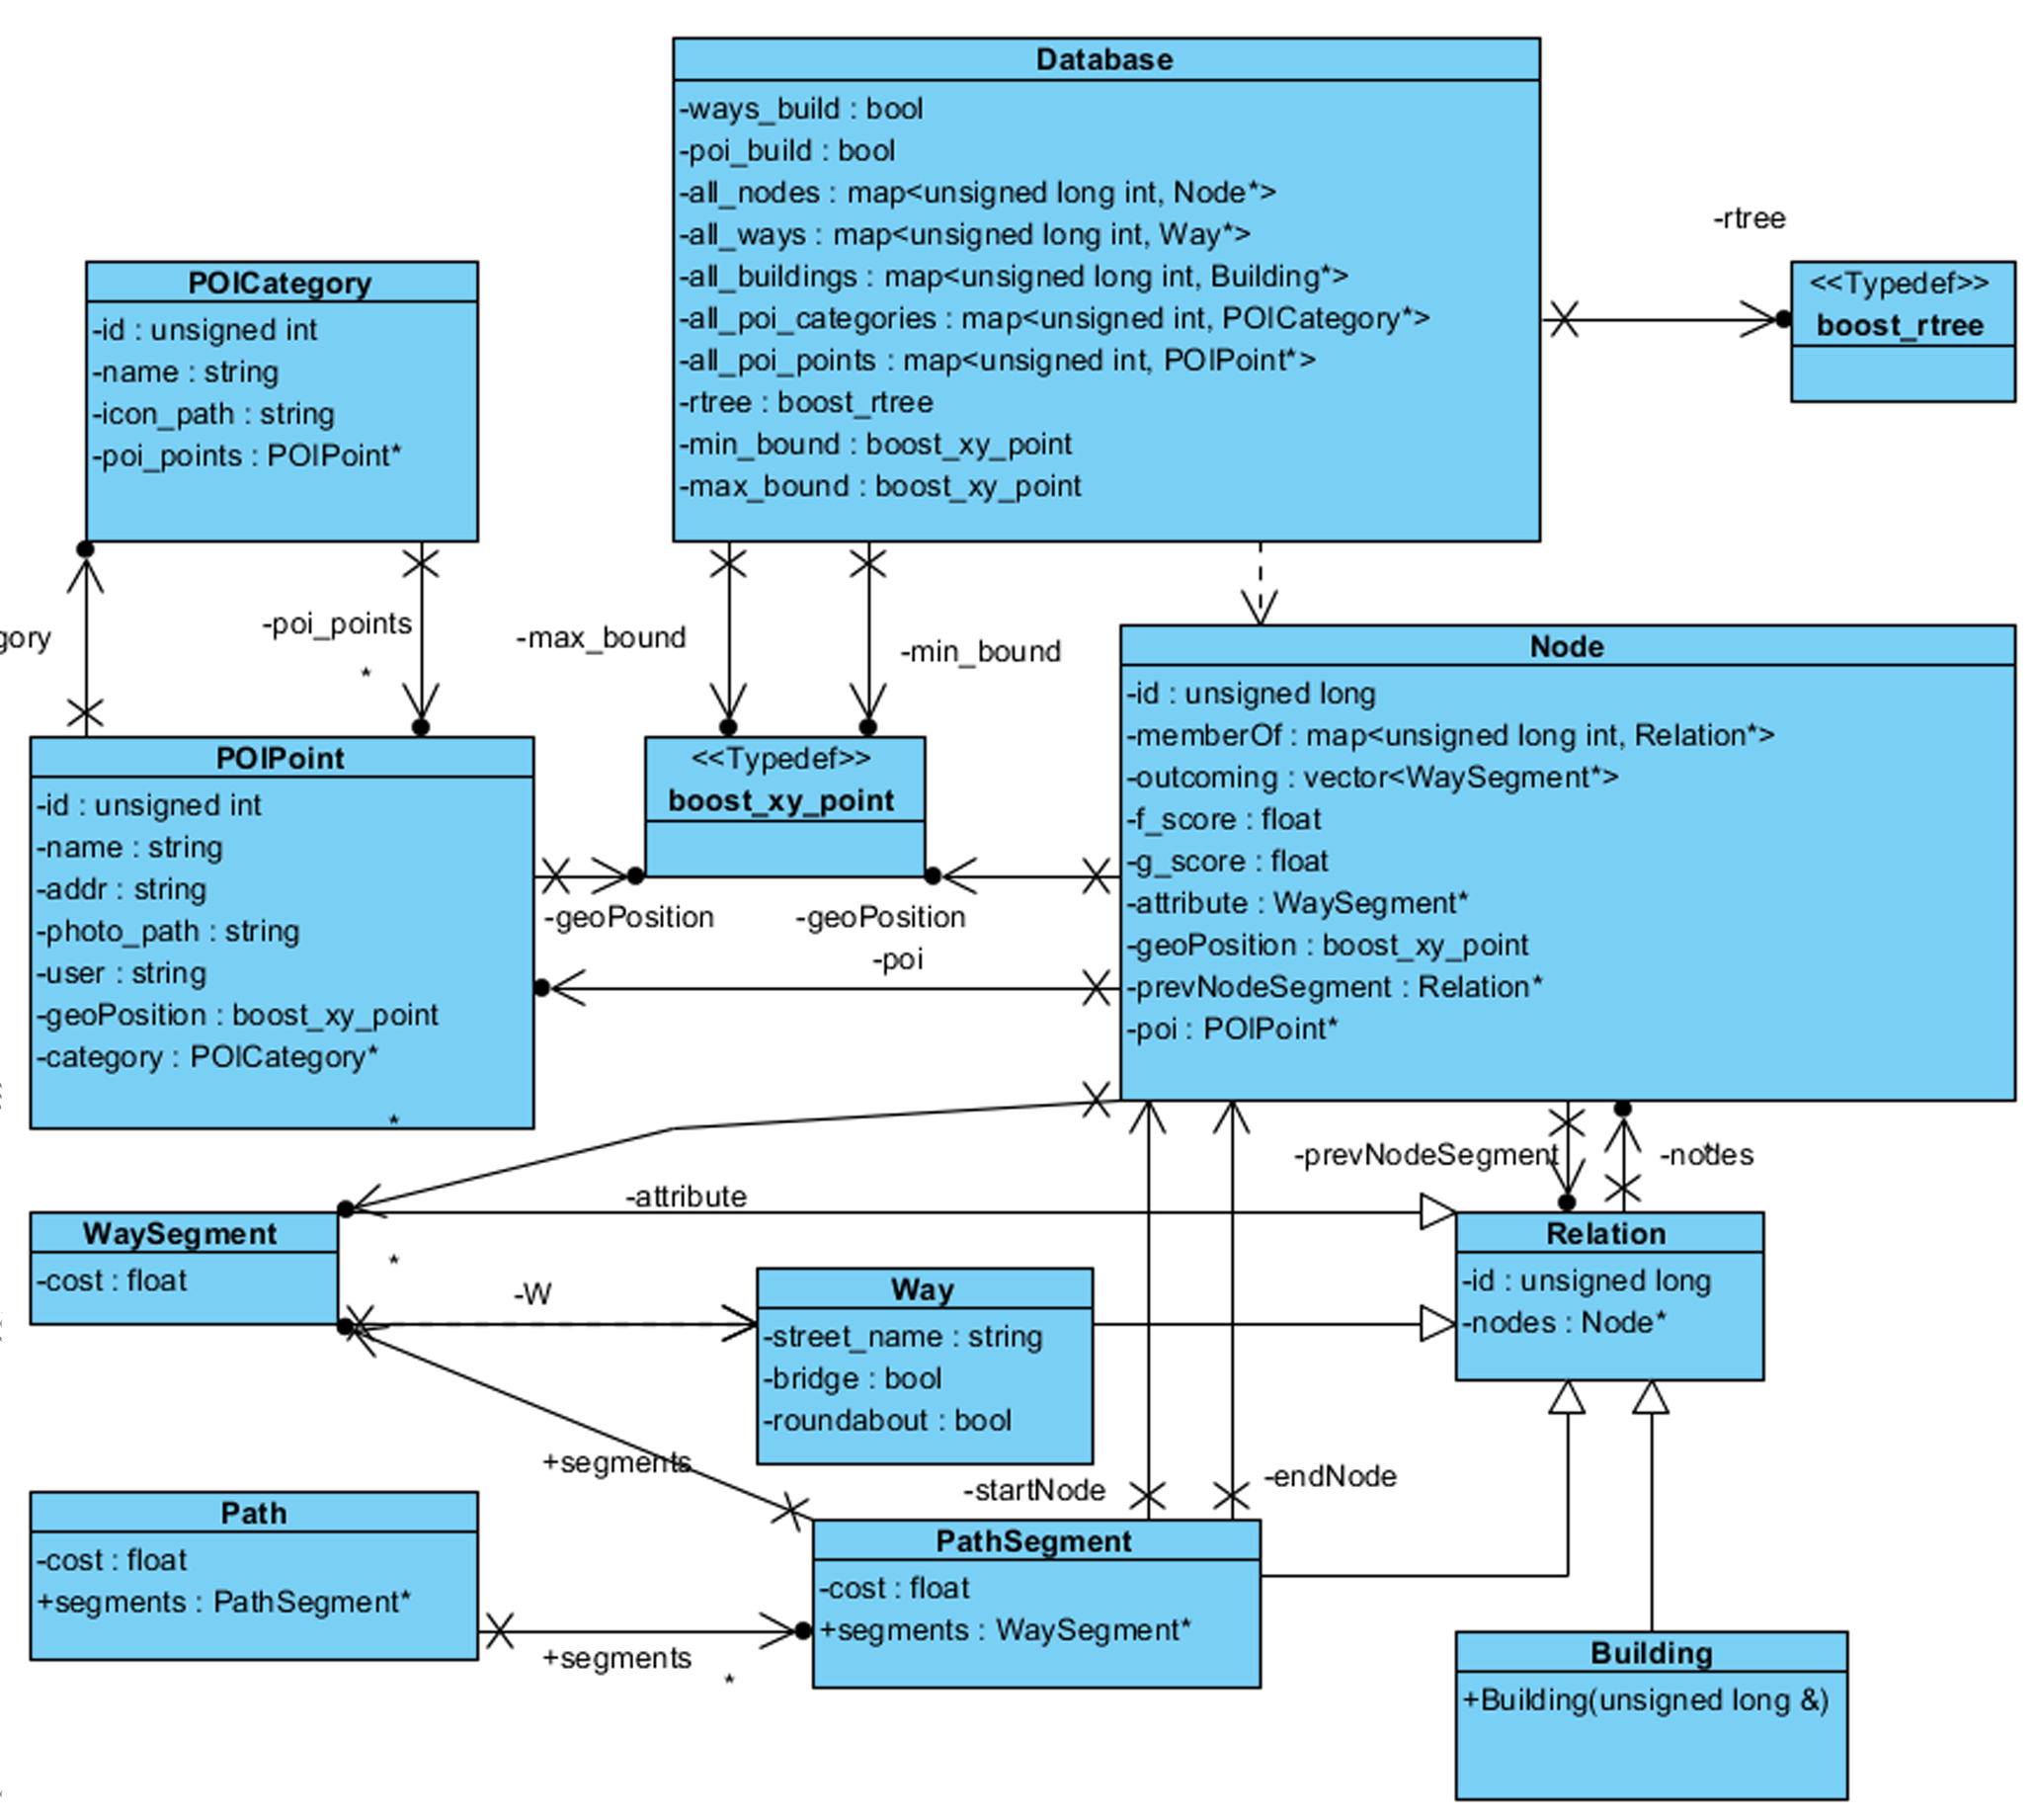
\includegraphics[height=4cm]{../photos/Class_Diagram.png}
 \caption{Class diagram}
 \label{fig:db_class}
 \end{figure}


\chapter{Path algorithms}
Finding the shortest path is one of the main problems in graph theory. It is a problem of finding a path between two nodes, where the sum of edge weights must be minimized. Graph can be undirected, directed or mixed.\\
The analogy with road maps can be clearly seen, where nodes correspond to intersections and road segments to edges on the graph. To properly represent oneway streets we use directed graph. The weight of each edge can be interpreted as a length of each road segment.\\ There are numerous algorithms that are able to found the shortest path. After initial research we narrowed the possible algorithms to:
\begin{itemize}
\item Dijkstra's algorithm
\item A* search algorithm
\item Bellman - Ford algorithm
\item Floyd - Warshall algorithm
\end{itemize}

From the user requirement analysis (section[]) we were able to identify the three main user requests involving path algorithms:
\begin{itemize}
\item find shortest path from point A to point B;
\item find shortest paths to all points of interest in a certain radius from point A (by foot or by car)
\item construct an itinerary from point A to B with points of interest in between (with max distance limit)
\end{itemize}

From identified requests, we can see that all of our path finding problems are actually problems of finding paths between points A and B. This are so-called single-pair shortest path problems. Analysing the algorithms listed above we determined that:
\begin{itemize}
\item Floyd - Warshall algorithm finds shortest paths between every pair of nodes in the graph
\item Dijkstra and Bellman - Ford algorithms find the shortest paths between source node and all other nodes on the graph (Bellman - Ford also permits negative weights)
\item A* algorithm finds the shortest path between the source and target node. 
\end{itemize}

All of the above algorithms encapsulate the result we need to find, but differing in how many unnecessary paths are also calculated. This subsequently mean longer calculation time, which we want to avoid. For this reasons we chose \textbf{A* path finding algorithm}.

\section{A*}
A* algorithm is one of the most popular path finding algorithms. Its ability to combine the benefits of Dijkstra's algorithm (favouring nodes close to the start node) and Best-First-Search algorithms (favouring nodes close to the target node) makes it efficient and accurate. 
\subsection{Process}
Algorithm works by traversing the graph node by node till it reaches the end node. At every step node with the lowest cost $(f(x))$ is selected. Calculation of the cost is what selected sets A* apart from other greedy best-first search algorithms. Cost is calculated as a weighted sum of:
\begin{itemize}
\item $g(n) - $\textit{exact cost} of the path from the starting point,
\item $h(n) - $\textit{heuristic estimated cost}.
\end{itemize}
Heuristics are used to control the A*'s behaviour. If $h(n)=0$ only distance from the start matters and we have 
normal Dijkstra algorithm. Because we do not know distance from node to end target, as we haven't traversed it yet, we have to estimate it. It is important not to overestimate the distance, as this can cause the algorithm to not found the shortest path. We decided to use air distance as a heuristic, as this guarantees that the actual distance will be equal or greater than that, so we never over-estimate it.

\section{Road snapping}
As described in the previous section A* algorithm enables us to find the shortest path between two nodes in a graph. This enforces the restriction of searching only on the locations of the nodes. This is a huge limitation, as on some parts of the map users point can be located far away from the closest node. To overcome this restriction we implemented \textbf{a road snapping function}.\\

Road snapping function finds the segment on which the perpendicular projection of user's point is closest to the user's point itself. Calculation of the perpendicular projection of a point on the segment is done using vectors and dot product between them. Algorithm used is described on website[]. It is worth mentioning that if the perpendicular projection of the point is outside of the interval between both nodes, it snaps to the border node. This can be seen on figure\ref{fig:db_snap} (left and right).

 \begin{figure}[h]
 \centering
 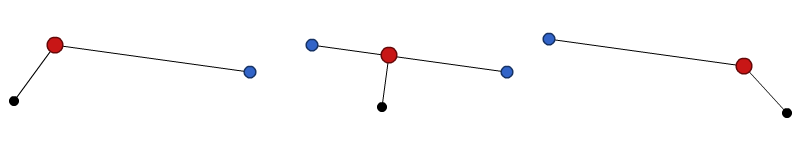
\includegraphics[width=0.8\linewidth]{../photos/snap_points.png}
 \caption{Snapping user point to border nodes (left,right) and snapping to perpendicular point where possible}
 \label{fig:db_snap}
 \end{figure}

 With this information we create a new mock node which represents the start point of our search. We connect this new node with the end nodes of the closest segment, making it possible to use it in A* algorithm. We repeat the same steps for the end point. After the search we remove all the nodes and edges we additional added, reverting back the graph to the same state as before the search.

  \subsection{Implementation in C++}
Road snapping function requires an extremely time consuming operation of finding close segments. We could have actually calculated the perpendicular projection on every WaySegment in the map and then among them find the smallest, but this would mean ten thousands of unnecessary calculations. Instead we used rtree data structure containing all the WaySegments implemented in \textit{Database class}. With this we were able to quickly find WaySegments whose bounding boxes intersect with our point. To compensate for areas, where roads are closely together, we implemented the search in small increasing steps. We start the with a small neighbourhood and gradually increasing it, until we find any intersecting WaySegments. This approach reduces the calculations of perpendicular projections from ten thousand to just a couple. The diagram of the proces is shown in the figure[]

\subsection{Implementation in Matlab}
Unfortunately Matlab does not have similar data structures capable of spatial filtering. To get the same end result we calculated the projection points on all the points and find the one with the minimal distance. To speed up the process of calculation we put the data in vectors and vectorize[matlab CITE] the code for calculation. The speed of the calculation turned out to be sufficient.

\section{Shortest path A $->$ B search}
Our algorithm for finding the shortest path between point A and point B is the collection of methods we already described. The whole process is shown on figure \ref{fig:ab_activity}.
 \begin{figure}[h]
 \centering
 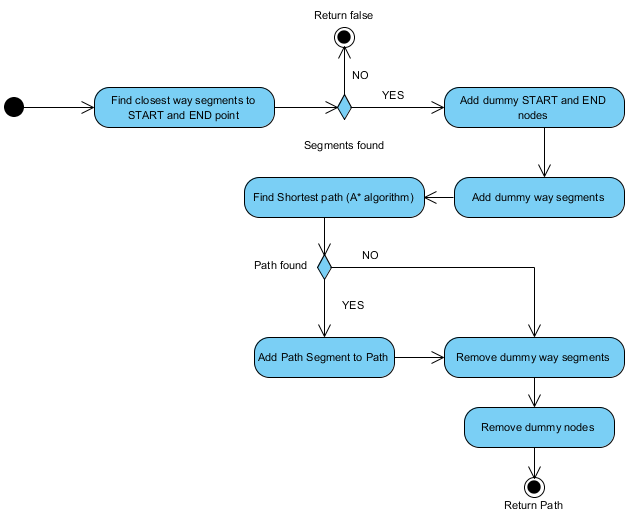
\includegraphics[width=0.7\linewidth]{../photos/shortest_path_ab_activity.png}
 \caption{Activity diagram of finding the shortest path between point A and B}
 \label{fig:ab_activity}
 \end{figure}

\section{Radius search}
\section{Bicycle search}
\chapter{Graphical User Interface}
\section{User Interface in C++}
\subsection{Framework choice}

For UI in this project we have chosen to use Qt Widgets Module. Qt features two technologies for creating desktop user interfaces. The first choice for this project was Qt Quick, since it provides the most appropriate functionality to mimic GoogleEarth web-application look and feel with fluid and dynamic user interface. However, the development process was very slow and difficult due to the fact that Qt Quick is rather new technology and not well-documented. It turned out to be more feasible to use older and more reliable technology, Qt Widgets. Qt Widgets are mature and feature rich user interface elements suitable for mostly static user interfaces. Besides, since Qt Widget are native C++ elements it is easier to merge UI with the application logic.
The application UI is connected to all other parts of the application through the class Logic.  The Logic handles all the data interchange between the UI, database and algorithms. In this was it is possible to split the application in separate parts. 

\subsection{Basic elements of UI}

The UI is straightforward and easy to use. There are two main parts - control panel and map. It is possible to extract three multiple cases of the application usage from the task: the search of Point-to-Point shortest path; the search of the destination in the given radius; the itinerary search with the middle point given as any from the category. Thus, the control contains three tabs corresponding to the three different functions. In each of them there are three options to enter the start and end point; you can either directly use geographical coordinates, choose from the category and POI, or by click on the map. Clicking on the map can have two effects: if you clock in the vicinity of the POI it will be chosen as start/end point, otherwise, just coordinates of the point clicked on the map will be set.
After user have chosen all the parameters of the search, the button "Go!" calls path searching algorithms. The important part is to check that inputs are valid and satisfy bounding conditions of the map. Then the result is displayed with graphical functions and text output.

\subsection{Editing the POI database}

The POI can be seen on the map as various descriptive icons according to the category they belong to. Once user clicks on one of the POI small widget appears with the details of the POI. If "Edit" button is pressed, you can edit any data belonging to the chosen POI. Besides user can add POI by choosing one on the options in the context menu, which appears with on-map mouse click. 
\section{Map Rendering in C++}
\section{Matlab}
\subsection{UI}
\subsection{library for maps}
\chapter{c++ vs matlab}




\begin{thebibliography}{99}

\bibitem{Bovey}
J. D. Bovey, M. M. Dodson,
The Hausdorff dimension of systems of linear forms
{\em Acta Arithmetica}
(1986) 337-358.

\bibitem{Cassels}
J. W. S. Cassels,
{\em An Introduction to Diophantine Approximation},
Cambridge University Press, 1965.

\bibitem{vec_matlab}


\end{thebibliography}


\end{document}
